\chapter{Event selection}
The experimental signature of our signal is the presence of two same-sign
prompt leptons and at least four jets (see figure~\ref{fig:TTbar_feynman}).

\begin{figure}[htb]
    \centering
    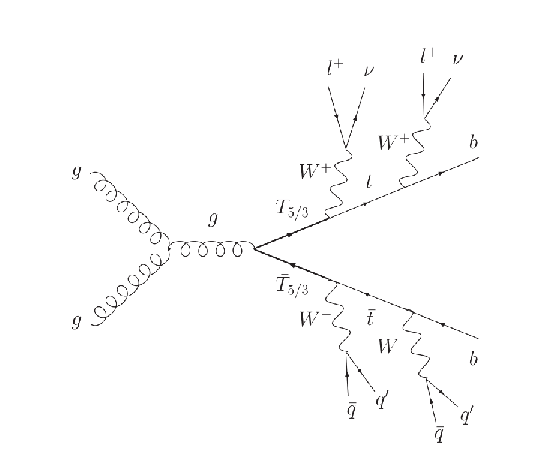
\includegraphics[width=\textwidth]{images/pdf/TTbar_feynman}
    \caption{Pair-production of the \TP, decaying into same-sign leptons and
    at least four jets.}
    \label{fig:TTbar_feynman}
\end{figure}

The backgrounds associated with this signal can be divided into three
categories:
\begin{description}
    \item[two same-sign prompt leptons] from rare SM processes.
    \item[opposite-sign leptons] whose charge is mismeasured, leading to a
        same-sign final state.
    \item[one prompt and one non-prompt lepton with the same charge] (or two
        non-prompt same-sign leptons). This background arises mainly from
        \ttbar events where one of the leptons comes from the decay of a
        $b$ quark, but is mistaken for a prompt lepton.
\end{description}


\begin{itemize}
    \item event cleanup and trigger
    \item exactly two same-sign leptons, rejecting events with three or more
        leptons
    \item quarkonia veto, with the invariant mass of the leptons greater
        than \unit[20]{GeV}
    \item \Z veto, with the invariant mass of the \E\E and \M\M pairs not in
        the 76-106 window. Note that this selection is not needed for \E\M
        events.
    \item at least four jets
\end{itemize}

